\chapter{Architettura della gamificazione}
Abbiamo quindi visto come costruire un sistema gamificato, quali sono i suoi elementi e che risultati può produrre. Cerchiamo ora di riorganizzare tutto in una vera e propria architettura che può essere usata in ambito educativo.

\section{Obbiettivi del progetto}

Il progetto vuole realizzare una WebApp che aiuti gli educatori, che siano scolastici oppure di discipline sportive, a impostare i propri insegnamenti con la tecnica di gamificazione, in modo da rendere l'insegnamento le più interessante e coinvolgente agli occhi dei frequentanti.\\
\\
In particolare:\\
 Un educatore può organizzare le proprie lezioni secondo le tecniche tipiche di gamificazione. L'organizzazione delle lezione sarà disposto a "missioni" dove completato un determinato numero di missioni si conclude un livello, oppure unità didattica.
Inoltre l'educatore può predisporre delle "missioni secondarie" non obbligatorie, pensate come delle sfide, tipicamente più difficili dei compiti assegnati normalmente. Se completate lo studente sarà ricompensato in qualche maniera, tipicamente con punti extra per l'esame finale.
Oltre a ciò un professore può per ogni studente dare le proprie valutazioni riguardante i compiti assegnati e in generale riguardo al periodo scolastico.\\
\\
Uno studente può registrarsi per iscriversi ad una classe. Una volta autenticato può consegnare i propri compiti e visualizzare le valutazioni ricevute. Più incarichi vengono svolti più vengono assegnati punti allo studente che potrà utilizzarli per personalizzare un avatar virtuale.\\
\section{Analisi SWOT}

Utilizziamo l'analisi SWOT per valutare punti di forza, debolezze, opportunità e minacce di questo progetto.

\textbf{Punti di forza:}
\begin{itemize}
  \item Mette sotto un'altra luce l'insegnamento agli occhi degli studenti che saranno più familiari con la struttura che avrà l'insegnamento poichè ricorda molto la struttura di diversi videogiochi.

  \item Facilita il controllo da parte dell'educatore in quanto potrà vedere quali missioni sono state completati da quali studenti, con la stessa facilità che è assegnare un compito per casa.
\end{itemize}

\textbf{Debolezze:}
\begin{itemize}
  \item In certi scenari dove c'è comunque bisogno di una certa supervisione alla consegna degli incarichi per accertarsi della correttezza dei compiti. Ad esempio in quei compiti dove non c'è una risposta precisa come la consegna di un tema scritto oppure l'esecuzione di 20 tiri liberi dalla linea di tre punti nel basket.


%  in ambito sportivo non può essere utilizzato a pieno o come a scuola xk serve più supervisione nello sport si potrebbe mettere cose per caricare video.
 % qua la AI potrebbe risolvere il problema
\end{itemize}

\textbf{Opportunità:}
\begin{itemize}
  \item Migliora il controllo a distanza degli incarichi assegnati agli studenti.

  \item Possiblità di diffusione in licei sportivi dove vengono insegnati più sport contemporaneamente permettendo di sfruttare al meglio la struttura non unicamente sequenziale che il progetto può offrire.
\end{itemize}

\textbf{Minacce:}
\begin{itemize}
  \item La piattaforma gamificata potrebbe non essere utilizzata da educatori scolastici per la sua non convenzionalità.
\end{itemize}

\section{User stories}

Raccogliamo quindi delle user story per tradurle in requisiti funzionali e non funzionali.\\
\\
\Large{User story 1}\\
Come professore, voglio avere un posto dove poter vedere tutti i compiti dei miei studenti cosi posso capire il grado generale di comprensione degli studenti.\\
\\
\Large{User story 2}\\
Come professore, voglio avere la possibilità di organizzare le lezioni per argomento così da poter tenere ordinate le lezioni e creare una sequenza naturale degli argomenti.\\
\\
\Large{User story 3}\\
Come professore, voglio avere una raccolta delle lezioni ed esercizi da assegnare così ogni anno sono già pronte e posso migliorarle invece che ripensarle da zero.
\section{Requisiti funzionali}
\subsection{Untente anonimo}

\textbf{RF1 Registrazione}

Il sistema deve permettere ad un utente di registrarsi al sistema compilando un form dove sono chiesti: nome, cognome, indirizzo mail, password (chiesta due volte per evitare errori), studente o professore.\\
\\
\textbf{RF2 Autenticazione}

Il sistema deve permettere all'utente di autenticarsi inserendo indirizzo email e password.\\
\\
\textbf{RF3 Conferma email}

Il sistema invierà all'email inserita in RF1 per confermare l'indirizzo email. La conferma avverrà all'apertura della mail.\\
\\
\textbf{RF4 Recupero password}

Il sistema deve permettere agli utenti di recuperare la propria password  cambiandola.
\subsection{Professore}

\textbf{RF5 Creazione di una classe}

Il sistema deve permettere i professori di raggruppare gli studenti in classi. Al professore verrà mostrata una pagina iniziale dove può dare il nome alla classe e tutte le informazioni relative ad essa, come indirizzo di studio e nome della scuola. Una volta completata la compilazione il sistema fornirà un link dalla quale gli studenti potranno registrarsi.\\
\\
\textbf{RF6 Creazione unità didattica}

Il sistema darà la possibilità al professore di creare delle unità didattiche. Ogni unità didattica contiene almeno sequenza di missioni con la possibilità di introdurre missioni secondarie. L'idea è ogni unità didattica sia un macro argomento di lezione, come ad esempio la statistica. Ogni sequenza di missioni sia un argomento, come la distribuzione di Poisson. Ogni missione rappresenta una serie di esercizi che dovrebbe scalare in difficoltà. Le missioni secondarie sono compiti facoltativi tipicamente più impegnativi.

Il professore dalla pagina principale della classe avrà l'opzione di creare una nuova unità didattica. A questo punto una finestra gli chiederà se vuole inserire una unità didattica esistente, prese da una raccolta di tute le unità didattiche del professore, oppure crearla da zero. Una volta creata la potrà popolare con tutte le missioni che desidera.\\
\\
\textbf{RF7 Creazione missioni}

Il sistema, dopo aver seguito i passi indicati in RF2, avrà l'opzione di inserire le missioni all'interno delle unità didattiche. Per ogni missione il professore potrà inserire delle dispense, video lezioni e dei compiti. La schermata avrà una finestra principale e un pannello laterale. Nella finestra principale saranno mostrati in ordine la videolezione seguita dalla dispensa e infine i compiti assegnati che dovranno essere consegnati per il completamento della missione da parte degli studenti. Nel pannello laterale invece il professore scriverà i meta dati della missione, come titolo, di cosa tratta, quale livello cognitivo secondo la piramide di Bloom soddisfa e quali missioni devono essere completate prima di poter completare la missione che si sta creando, in modo da poter creare una sequenza di queste.\\
\\
\textbf{RF8 Gestione missioni}

Il sistema dalla schermata principale della classe mostrare a lato le unità didattiche predisposte. Selezionando una di queste aprirà l'elenco delle missioni al suo interno. Ogni missione avrà accanto una casella che se spuntata la pubblica per la visione degli studenti.\\
\\
\textbf{RF9 Valutazione delle missioni}

Il sistema dalla selezione effettuata in RF4 verranno visualizzate tutte le missioni. Cliccando una missione si aprirà una finestra che farà vedere la missione come la vedrebbero gli studenti e descritta in RF3 e a lato avrà una lista degli studenti che hanno consegnato il compito. Cliccando uno studente si potrà visualizzare i files che ha caricato per la valutazione.
In alternativa si può dalla schermata della classe cliccare il nome di uno studente e visualizzare tutte le consegne di quello studente e valutarle da lì.\\
La valutazione dello studente sarà divisa in blocchi percentuali, ad esempio 0-20\% oppure 60-80\%. Ci saranno 5 divisioni che rappresenteranno il grado di successo della missione. Secondo il grado lo studente riceverà una ricompensa per il suo avatar migliore.\\
\\
\textbf{RF10 Visualizzazione andamento studente}

Il sistema dalla schermata principale della classe, cliccando uno studente, oltre a vedere tutte le sue consegne, per quelle valutate si vedrà anche la valutazione assegnata.

\subsection{Studente}

\textbf{RF11 Iscrizione ad una classe}

Il sistema cliccando il link per unirsi ad una classe aprirà una schermata che ci informerà che ci stiamo unendo alla classe.\\
\\
\textbf{RF12 Personalizzazione avatar}

Il sistema dalla schermata principale dello studente e cliccando la figura dell'avatar mostrata potrà entrare nel menù di personalizzazione. Al suo interno potrà cambiare l'aspetta del proprio avatar in termini di aspetto fisico e selezionare l'equipaggiamento che indossa.
L'equipaggiamento potrà essere ottenuto completando le missioni e in base alla valutazione riceverà un versione migliore di esso. Se la valutazione è bassa l'armatura o gli stivali o la spada di ricompensa saranno più logori. Se la valutazione è alta invece saranno più belli esteticamente.\\
\\
\textbf{RF13 Consegna missioni}

Dalla schermata principale dello studente, dall'elenco delle missioni è possibile cliccare una di esse per vedere il materiale caricato dal professore. In fondo alla pagina ci sarà una sezione dove è possibile caricare l'elaborato dei propri compiti.\\
\\
\textbf{RF14 Visualizzazione valutazioni}

Il sistema dalla schermata principale dello studente cliccando sull'avatar si aprirà la schermata dell'avatar. Dal lato destro sarà possibile personalizzarlo come descritto in RF9 ma a sinistra sotto l'avatar sarà visualizzabile un istogramma. Ogni colonna avrà un'etichetta associata al nome di una missione, che dovrebbe essere il nome degli esercizi assegnati nella missione. Ogni colonna farà vedere la valutazione della missione. La schermata dovrà emulare l'aspetto di una pagina di statistiche del personaggio, Es Forza 80 agilità 50 ecc...\\
\\
L'idea di fondo è che le statistiche sono legate all'equipaggiamento che però sarà migliore proporzionalmente alle valutazioni ricevute. Quindi più uno studente avrà valutazioni alte, più alta sarà la colonna della valutazione delle missioni, che rappresentano una statistica come forza, agilità e cosi via, migliore sarà l'aspetto dell'avatar dello studente poichè ha ricevuto un'equipaggiamento migliore per via della sua valutazione.
\section{Requisiti non funzionali}

\textbf{RNF1 Privacy}

Il sistema deve rispettare il regolamento europeo 2016/679 noto come GDPR (General Data Protection Regulation).\\
\\
\textbf{RNF2 Sicurezza}

\begin{itemize}
  \item La trasmissione dei dati deve essere sicura.
  \item I dati di accesso non devono essere salvati in chiaro.
  \item Un utente autenticato deve poter uscire dal proprio account
\end{itemize}

\textbf{RNF3 Portabilità}

Ogni funzione deve essere funzionante su browser: Chrome 18+, Chrome Mobile 18+, Safari 5.1+\\
\\
\textbf{RNF4 Prestazioni}

\begin{itemize}
\item La funzione di consegna missioni RF13 deve essere eseguita dal sistema al più in 10 secondi.

\item La funzione di creazione missioni RF7 deve essere eseguita dal sistema al più in 10 secondi.
\end{itemize}

\textbf{RNF5 Facilità d'uso}

\begin{itemize}
  \item Un utente deve essere in grado di registrarsi ed autenticarsi (RF1, RF2) senza addestramento in al più 10 minuti.

  \item Uno studente deve essere in grado di consegnare una missione (RF13) senza addestramento in al più 5 minuti.
\end{itemize}

\section{Use cases}
\textbf{Use case:} Registrazione\\
\textbf{Riassunto:} Descrive come l'utente anonimo effettua la registrazione come professore oppure studente.\\
\textbf{Descrizione:} \begin{enumerate}
  \item L'utente inserisce nome e cognome. [eccezione 1]
  \item L'utente inserisce email. [eccezione 2]
  \item L'utente inserisce due volte la password. [eccezione 3]
  \item L'utente indica di essere studente o professore. [eccezione 4]
  \item L'utente invia il form premendo il pulsante "Registrati". [eccezione 5] [eccezione 6]
  \item Appare su schermo la scritta registrazione completata.
\end{enumerate}
\textbf{Eccezioni: }\begin{enumerate}
  \item Il nome e/o il cognome non è valido (non soddisfa la regex " [A-Za-z] {3,20}"), il bordo del campo del form diventa rosso.

  \item L'indirizzo email non è valido (non soddisfa la regex " +0.+\..+"), il bordo del campo del form diventa rosso.

  \item Le due password non sono congruenti, il bordo del campo del form diventa rosso.

  \item Non è selezionata nessuna delle due opzioni, il bordo del campo del form diventa rosso.

  \item Vi è almeno un campo del form vuoto o non valido, appare in rosso la scritta "Compila correttamente il form".

  \item L'indirizzo email inserito è già utilizzato da un altro account, appare la scritta "Indirizzo email già utilizzato.
\end{enumerate}
\begin{figure}[h!]
  \centerline{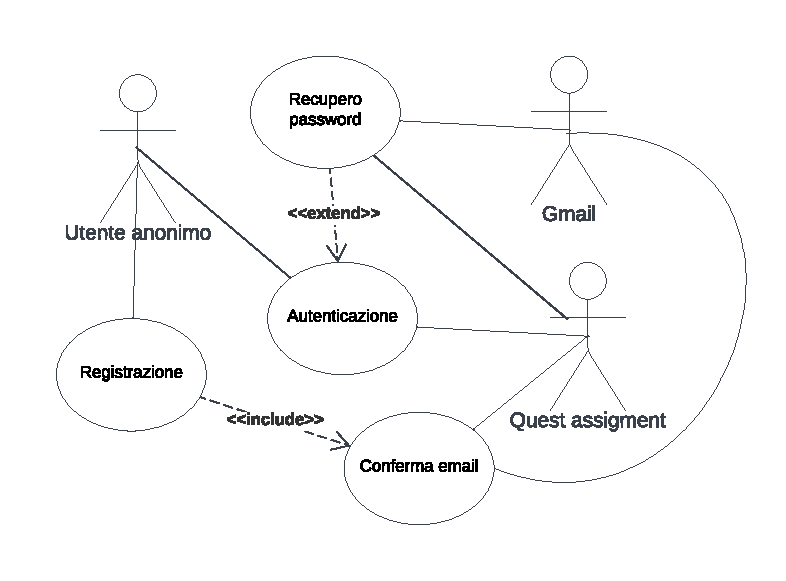
\includegraphics[trim={0 0.9cm 0 0.9cm},clip, angle=0,height=6.5cm,width=10cm]{figures/anonimo.pdf}}
  \caption{Diagramma Use case utente anonimo}
\end{figure}

\textbf{Use case:} Personalizzazione avatar\\
\textbf{Riassunto:} Una serie di parametri permettono la personalizzazione dell'aspetto dell'avatar dello studente.\\
\textbf{Descrizione:} \begin{enumerate}
  \item L'utente clicca l'immagine dell'avatar.

  \item L'utente visualizza un form aspetto fisico dove può scegliere: taglio di capelli, colore degli occhi, forma del viso, colore della pelle.

  \item L'utente visualizza un form equipaggiamento dove può selezionare: pettorina, elmo, stivali, pantaloni, arma. [eccezione 1]
\end{enumerate}
\textbf{Eccezioni: }\begin{enumerate}
  \item Se un campo è vuoto verrà mostrato un equipaggiamento di default che consiste in nessuna arma e indumenti da contadino.
\end{enumerate}

\textbf{Use case:} Consegna missioni\\
\textbf{Riassunto:} Permette all'utente di consegnare i compiti di una missione selezionata.\\
\textbf{Descrizione:} \begin{enumerate}
  \item L'utente clicca dall'elenco di missioni la missione di cui vuole consegnare il compito.

  \item L'utente trascina lo zip da consegnare in un riquadro. [eccezione 1]

  \item L'utente clicca il pulsante "Consegna missione". [eccezione 2]
\end{enumerate}
\textbf{Eccezioni: }\begin{enumerate}
  \item Il file supera i 2 Gb, appare un messaggio di errore "File troppo grande".
  \item Non è stato incluso nessun file, il pulsante diventa rosso e appare una scritta "carica elaborato".
\end{enumerate}

\textbf{Use case:} Visualizza valutazioni\\
\textbf{Riassunto:} Vengono visualizzate le valutazioni delle missioni con un istogramma con un numero corrispondente alla valutazione sopra la colonna corrispondente\\
\textbf{Descrizione:} \begin{enumerate}
  \item L'utente clicca l'immagine dell'avatar.

  \item L'utente visualizza sotto il proprio avatar un istogramma con tante colonne quante missioni consegnate e con il numero corrispondete alla valutazione sopra alla colonna.
\end{enumerate}

\begin{figure}[h!]
  \centerline{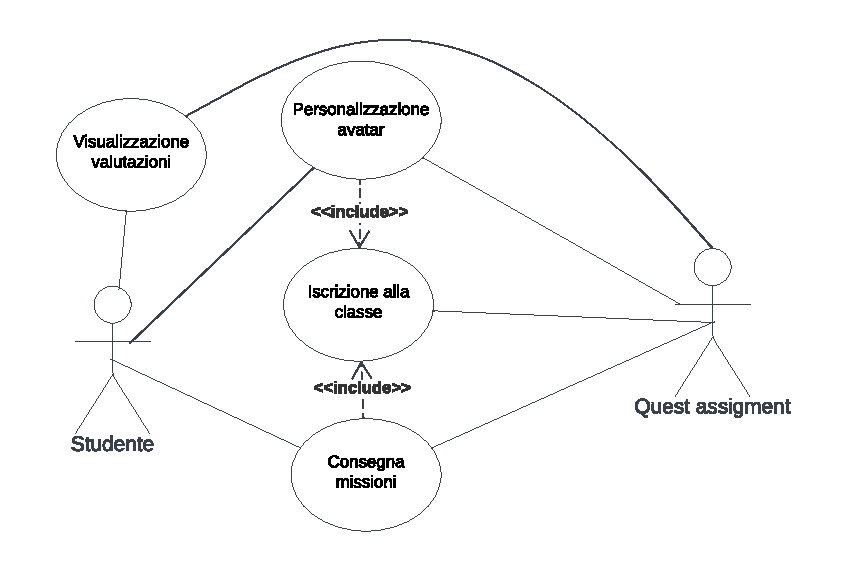
\includegraphics[trim={0 0.9cm 0 0.6cm},clip,height=7cm,width=10cm,angle=0]{figures/studente.pdf}}
  \caption{Diagramma Use case studente}
\end{figure}









\textbf{Use case:} Creazione classe\\
\textbf{Riassunto:} Questo use case descrive come avviene la creazione e popolazione di una classe.\\
\textbf{Descrizione:} \begin{enumerate}
  \item Il professore clicca il pulsante crea nuova classe.

  \item Il professore inserisce l'anno della classe

  \item Il professore inserisce l'indirizzo di studio della classe

  \item Il professore inserisce la sezione della classe.

  \item Il professore clicca il pulsante "Crea classe". [eccezione 1]

  \item il professore visualizza un link che deve inviare agli alunni.

  \item il professore visualizza man mano che gli studenti si unisco tutti i nomi di chi si aggiunge.

  \item Il professore clicca il pulsante "Ammetti" o "Rifiuta" per ammettere gli studenti giusti.
\end{enumerate}
\textbf{Eccezioni: }\begin{enumerate}
  \item Vi è almeno un campo del form vuoto o non valido, appare in rosso la
  scritta ”Compila correttamente il form".
\end{enumerate}














\begin{figure}[h!]
  \centerline{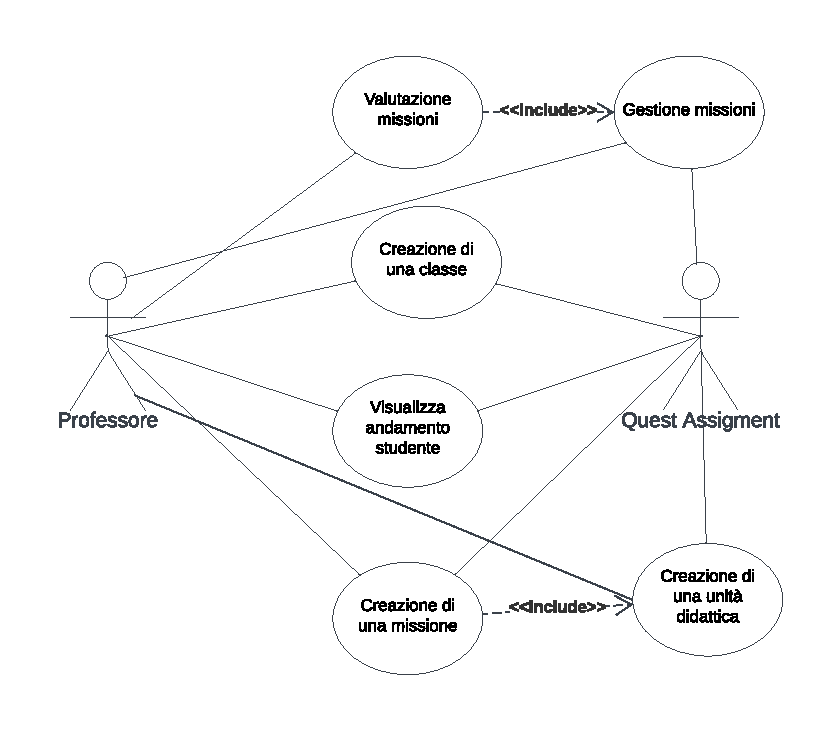
\includegraphics[trim={0 0.9cm 0 0.9cm},clip ,height= 7cm,width=10cm,angle=0]{figures/professore.pdf}}
  \caption{Diagramma Use case professore}
\end{figure}
















\section{Analisi del contesto}

Andiamo adesso a condurre un'analisi del contesto. Vogliamo identificare gli attori del sistema i sistemi esterni, paritari e subordinati. Distingueremo i flussi principali di dati e riassumeremo tutto in un diagramma di contesto.

\subsection{Utenti e sistemi esterni}

\textbf{Utente anonimo:} L'utente anonimo è l'attore qualsiasi che accede al sistema. Egli può registrarsi, autenticarsi, confermare la mail e recuperare la password.

\textbf{Professore: }Il professore è l'attore che ha lo scopo di insegnare agli studenti caricando le proprie lezioni e assegnando incarichi. Egli può: creare classi, creare missioni, creare unità didattiche, visualizzare i risultati degli studenti, valutare una missione, gestire le missioni.

\textbf{Studente: }Lo studente è l'attore che accede al sistema con lo scopo riceve il materiale di studio fornito dal professore e consegnare i propri compiti. Egli può: iscriversi ad una classe, visualizzare le sue valutazioni, personalizzare il proprio avatar, consegnare missioni.

\textbf{Gmail: }Gmail è il sistema esterno subordinato utilizzato per richiedere invio di mail come in RF3 e RF4.

\textbf{MongoDB:} MongoDB è il sistema esterno paritario utilizzato per archiviare tutte le infomazioni che hanno bisogno di una memorizzazione non volatile.

\begin{figure}[h!]
  \centerline{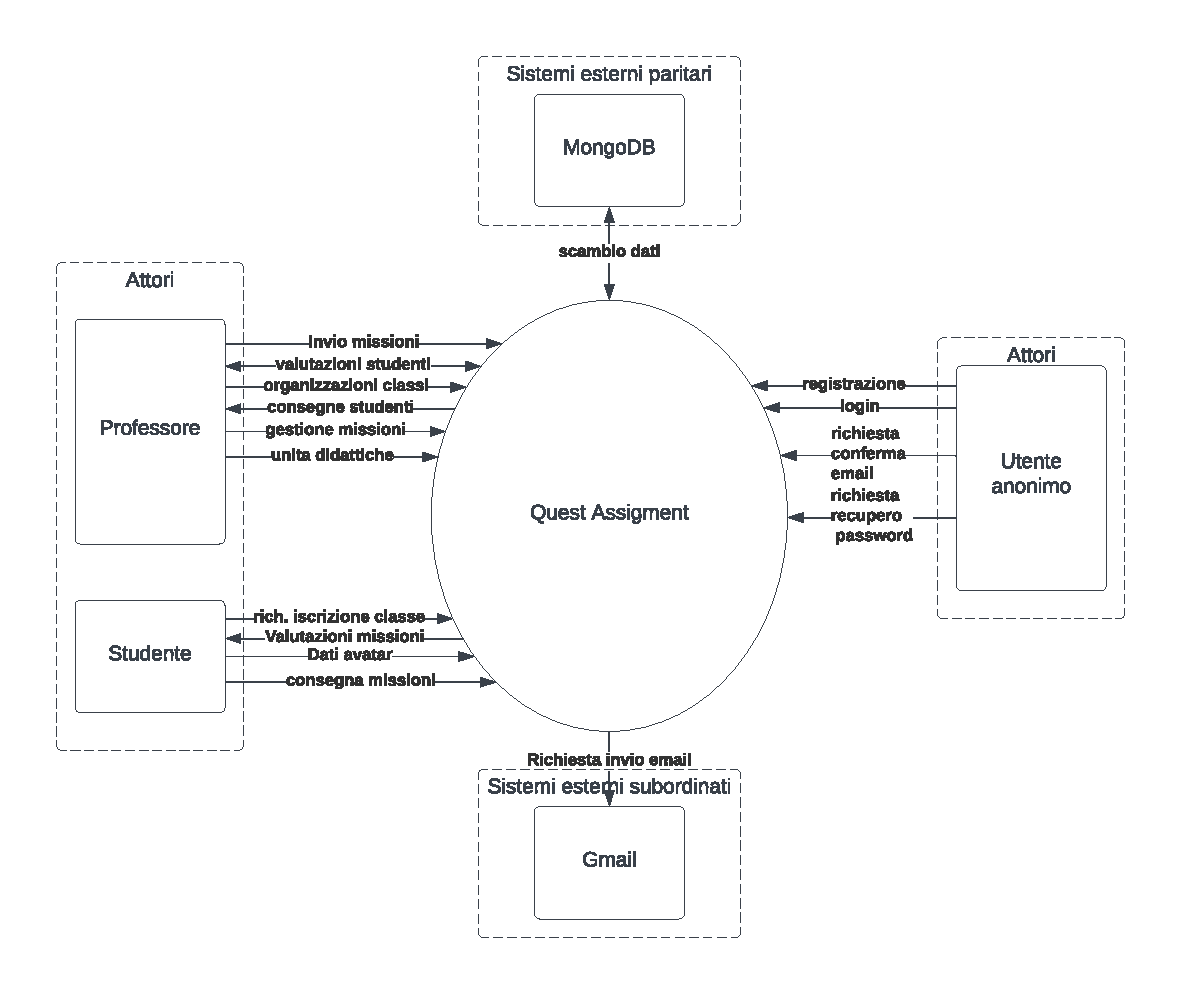
\includegraphics[trim={1cm 1cm 1cm 1cm},clip,height = 9 cm, width= 13 cm]{figures/contesto.pdf}}
  \caption{Diagramma di contesto}
\end{figure}

\section{Componenti}

I componenti che ci sono necessari sono: L'homepage, pagina degli studenti, pagine dei professori, gestione avatar, gestione missioni e autenticazione.\\
\\
L'homepage si occupa di registrare chiedendo agli utenti nuovi password e indirizzo mail e il ruolo che ricoprono. Una volta registrati indirizzano i professori e studenti nelle rispettive pagine dove si autenticheranno.\\
\\
L'autenticazione riceve le nuove registrazioni dalla homepage e fornisce le informazioni necessarie all'email sender per costruire l'email di conferma che verrà spedita agli utenti appena registrati. Inoltre si occupa di controllare i dati di login che arrivano dalle pagine di studenti e professori.\\
\\
La pagina degli studenti richiede allo studente il login e gli permette di visualizzare e caricare le missioni assegnate che verranno gestite dalla gestione missioni. Inoltre possono modificare l'aspetto del loro avatar e visualizzare le valutazioni delle missioni.\\
\\
La pagina dei professore richiede agli stessi il login e possono caricare le missioni da assegnare agli studenti. Inoltre possono fornire le valutazioni di quest'ultime per la visione degli studenti.\\
\\
La gestione delle missioni provvede a trasformare gli incarichi del professore come missioni di gioco per il meccanismo della gamificazione. Ovvero assegna le ricompense alla singola missione e rende questa informazione disponible alla gestione avatar in modo da poter far vedere all'utente gli elementi personalizzabili corretti.\\
\\
La gestione dell'avatar gestisce le modifiche degli avatar e fa vedere gli equipaggiamenti corretti grazie alle informazioni che riceve dalla gestione missioni e il grado di bellezza dalle valutazioni fornite dal professore.\\
\\
L'email sender si preoccupa di mandare la mail di registrazione.


\begin{figure}[h!]
  \centerline{\includegraphics[height=18cm, width=10cm, angle=270]{figures/componenti.pdf}}
  \caption{Diagramma dei componenti}
\end{figure}

\newpage
|..............................|\\
V Da cancellare V

\cite{learing}
\cite{approach}
\cite{medicina}
\cite{romanzi}
\cite{Dale}
\cite{teaching}
\cite{distribuzione}
\cite{stili}
\cite{game}
\newpage
